\section{Solutions on the market}

The following chapter presents the two most popular solutions used in the context of service meshes: \textsc{Istio} and \textsc{Linkerd}. Both technology solutions have in common that they are based on \textsc{Kubernetes}. While \textsc{Linkerd} requires \textsc{Kubernetes}, \textsc{Istio} could also rely on virtual machines.

Service meshes that use \textsc{Kubernetes} extend the functionality by abstracting concepts like automatic sidecar injection. This would be also possible without service meshes, but significantly more complex and less automated.

\subsection{Istio}

As illustrated in figure \ref{fig:arch-istio}, \textsc{Istio} uses a basic control and data plane architecture, as explained in chapter \ref{chap:mesh-architecture}. For the data plane, it uses the sidecar pattern by using \textsc{Envoy} proxies. \textsc{Envoy} a high-performance proxy that already brings features like service discovery, load balancing, circuit breaking and many more \cite{istio-docs-arch}.

\textsc{Istiod} (Istio daemon) provides management for service discovery, configuration and certificates. It converts routing rules into \textsc{Envoy}'s configuration format and also directs the traffic to the sidecar proxies \cite{istio-docs-arch}.

\begin{figure}
    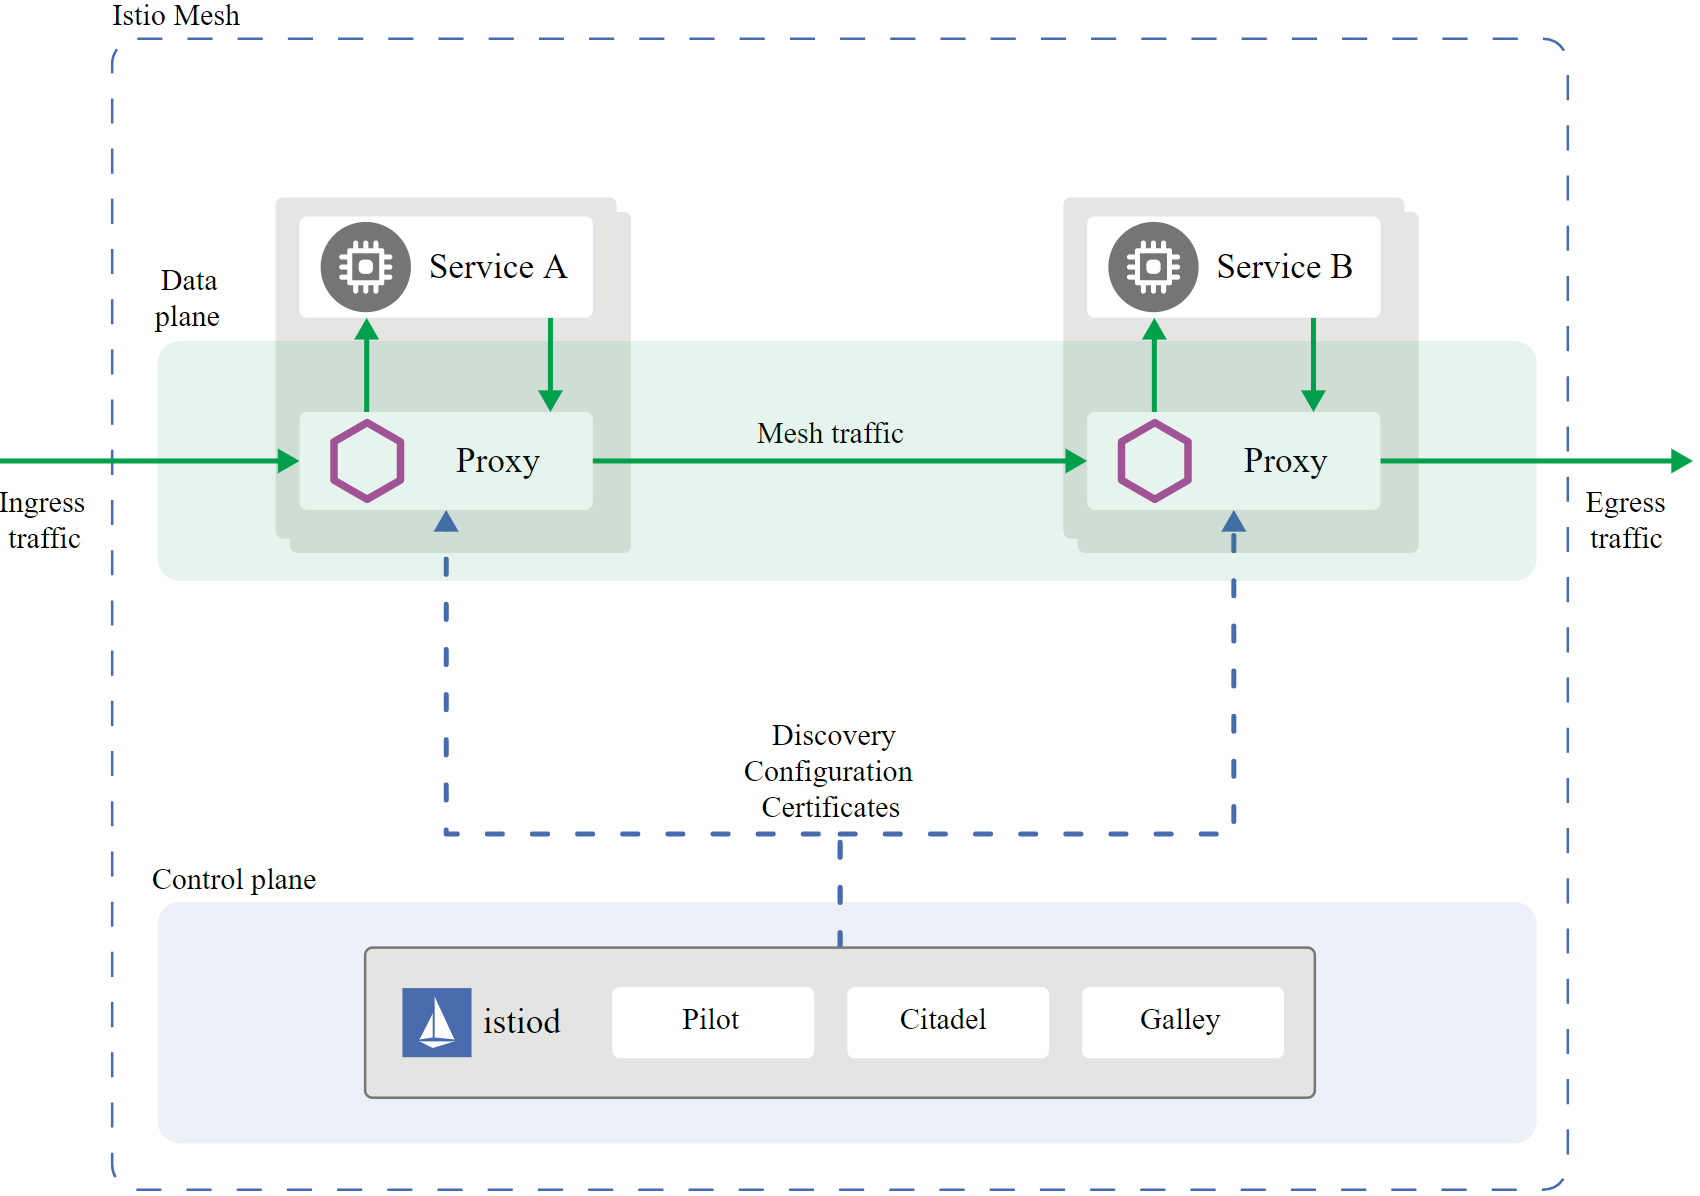
\includegraphics[width=\columnwidth]{img/istio_architecture.png}
    \caption{Architecture of \textsc{Istio} \cite{istio-docs-arch}}
    \label{fig:arch-istio}
\end{figure}

\subsection{Linkerd}
\label{linkerd}
According to \textsc{Linkerd}'s documentation \cite{linkerd-docs-arch}, \textsc{Linkerd} also uses a basic control and data plane architecture, as explained in chapter \ref{chap:mesh-architecture}. It also uses the sidecar pattern, but has implemented an own proxy solution named \textsc{Linkerd2-proxy}. \textsc{Linkerd} developers rate \textsc{Envoy} as too complex \cite{linkerd-docs-no-envoy}, which is why they decided to implement their own solution, which they call a "micro-proxy". 
Unlike \textsc{Istio}, \textsc{Linkerd} does not handle ingress traffic. It works in conjunction of every ingress controller of choice, e.g. \textsc{nginx} or \textsc{traefik} \cite{linkerd-docs-faq}.

As illustrated in figure \ref{fig:arch-linkerd}, each \textsc{linkerd-proxy} has access to two components: \textsc{identity} and \textsc{destination}.

\textsc{destination} is a lookup-service, where each proxy is able to check where exactly to send requests. \textsc{identity} provides a certificate authority.

While injecting a sidecar proxy on an application service, a route \textsc{/metrics} at port 4191 is exposed to provide log messages and metrics for \textsc{Prometheus}, which is a central logging and monitoring instance which is often used with \textsc{Kubernetes} \cite{linkerd-docs-arch}.

\begin{figure}
    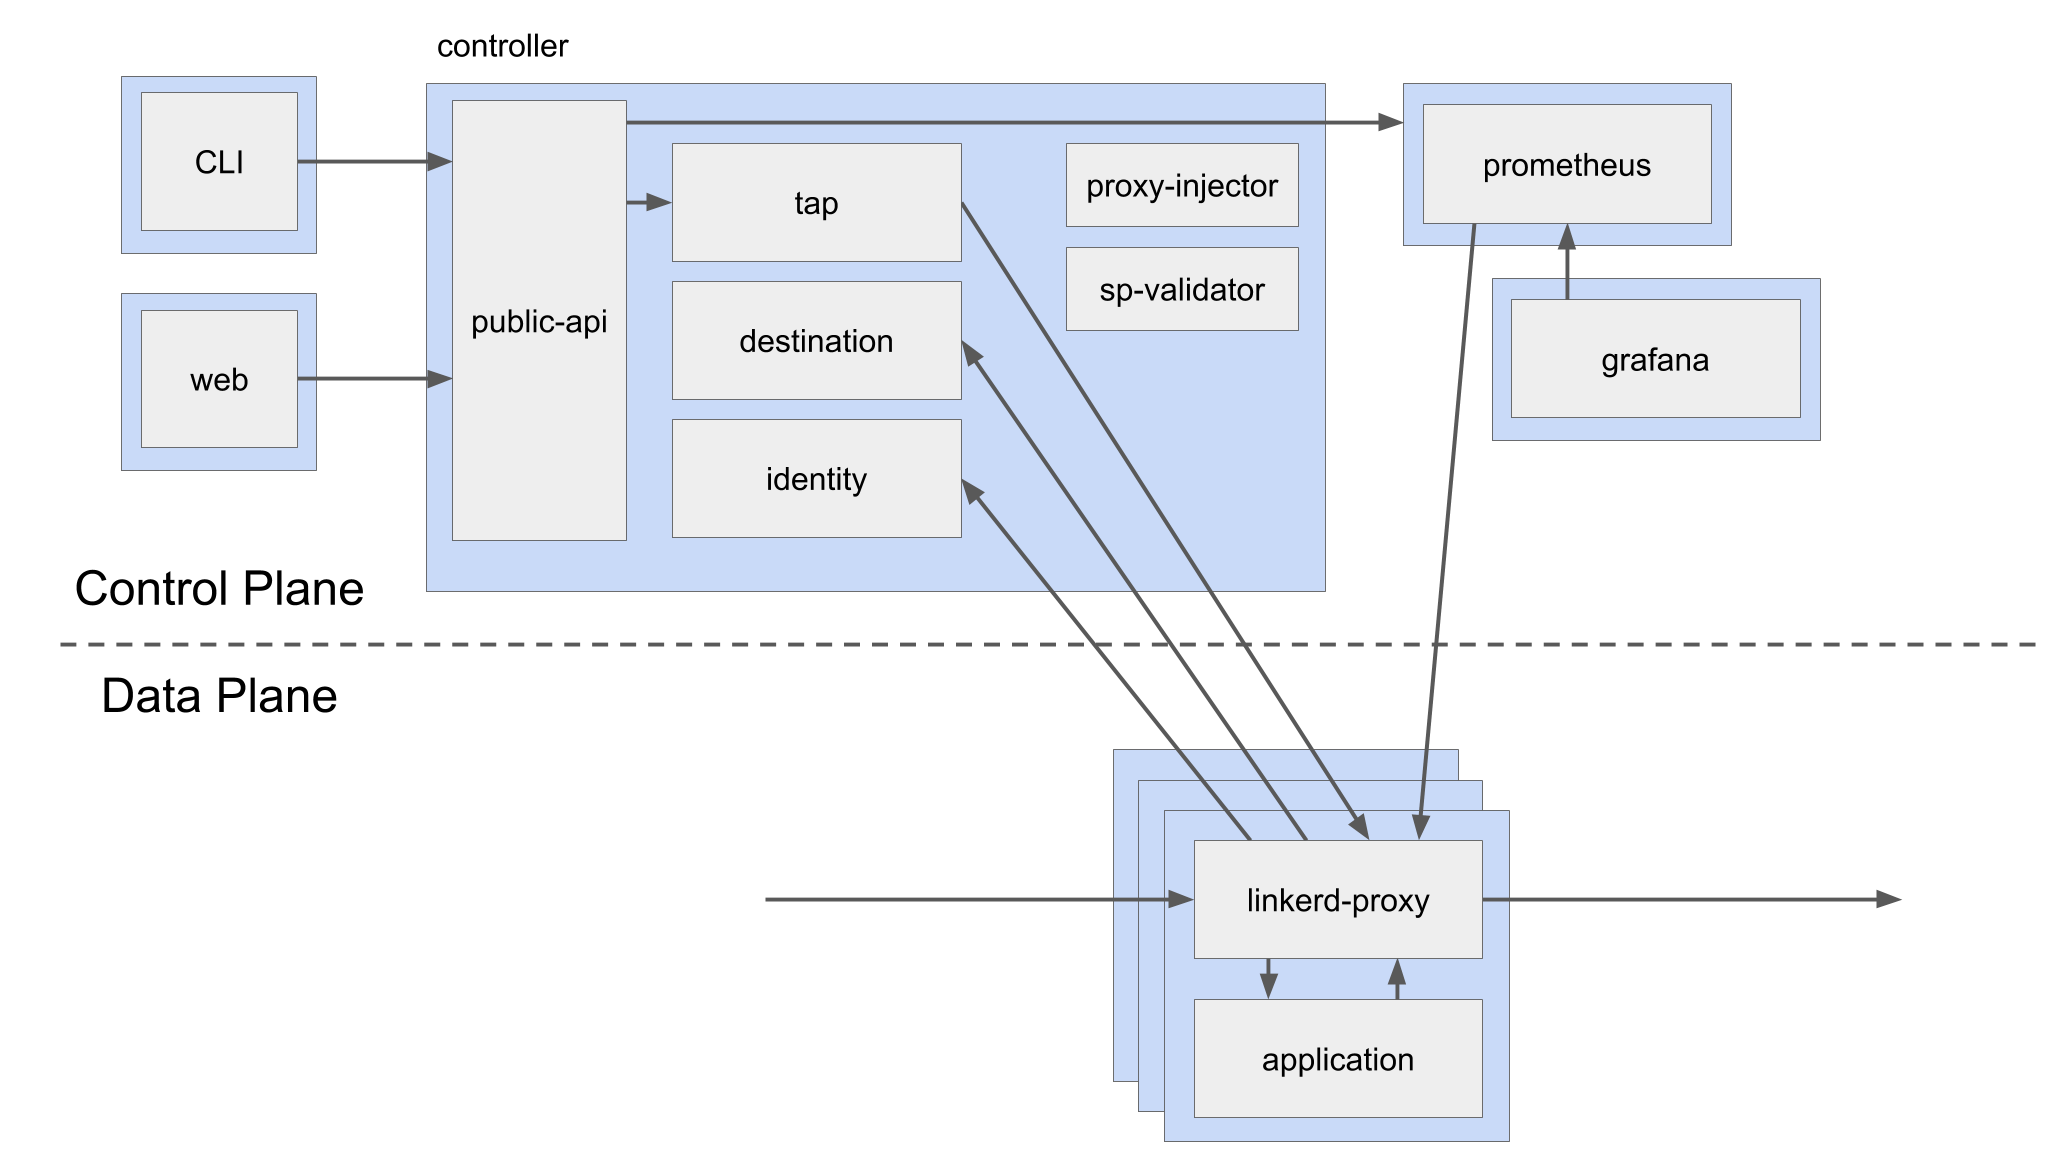
\includegraphics[width=\columnwidth]{img/linkerd_architecture.png}
    \caption{Architecture of \textsc{Linkerd} \cite{linkerd-docs-arch}}
    \label{fig:arch-linkerd}
\end{figure}

\subsection{Comparison}

As stated before, two very popular solutions for service meshes are \textsc{Linkerd} and \textsc{Istio}. Table \ref{tab:istio-linkerd} summarizes the key aspects of both tools, according to \cite{linkerd-github}, \cite{istio-github}, \cite{istio-linkerd-compare-1} and \cite{istio-linkerd-compare-2}:

\begin{table}
\centering

\begin{tabular*}{\columnwidth}{c|c|c}
                                 & Istio                                                                                                              & Linkerd     \\\hline
Initiators & \begin{tabular}[c]{@{}c@{}}Lyft, IBM,\\Google\end{tabular}                                                          	& \begin{tabular}[c]{@{}c@{}}Buoyant, Cloud Native\\Foundation\end{tabular}                                                           \\\hline
License                 & \multicolumn{2}{c}{Apache 2.0}                                                                                                          \\\hline
Runs on                          & \begin{tabular}[c]{@{}c@{}}Kubernetes,\\VMs\end{tabular}                                                           & Kubernetes  \\\hline
Sidecar proxy                    & \multicolumn{2}{c}{Yes}                                                                                                          \\\hline
Supports mTLS                    & \multicolumn{2}{c}{Yes}                                                                                                          \\\hline
Certificate management           & \multicolumn{2}{c}{Yes}                                                                                                          \\\hline
Authentication and authorization & \multicolumn{2}{c}{Yes}                                                                                                          \\\hline
Blue/Green deployment            & \multicolumn{2}{c}{Yes}                                                                                                          \\\hline
Circuit breaking                 & Yes                                                                                                                & No          \\\hline
Fault injection                  & \multicolumn{2}{c}{Yes}                                                                                                          \\\hline
Rate limiting                    & \multicolumn{2}{c}{Yes}                                                                                                          \\\hline
Monitoring                       & \multicolumn{2}{c}{Yes, with Prometheus}                                                                                         \\\hline
Complexity                       & High                                                                                                               & Low         \\\hline
Starts on GitHub \cite{linkerd-github} \cite{istio-github}              & 26.2k & 6.6k        \\\hline
Open issues on GitHub \cite{linkerd-github} \cite{istio-github}                 & 817                                                                                                                & 257         \\\hline
Documentation                    & ++                                                                                                                 & +          
\end{tabular*}
\vspace{0.25mm}
\caption{Comparison between Isto and \textsc{Linkerd}}
\label{tab:istio-linkerd}
\end{table}


%
%
% Mehr Erklärung zu Linkerd?
%
%

From an operators perspective, \textsc{Istio} and \textsc{Linkerd} look quite similar. After installing the service mesh, there are two main usage aspects: One the one hand, operators need to inject sidecar proxies in the pods of the microservice. On the other hand, they need to apply pluggable resources in YAML format, that could define policies like the usage of TLS.

By executing the command listed in \ref{lst:istio}, all deployments from namespaceA automatically get a sidecar proxy injected, while listing \ref{lst:linkerd} shows the injection command of a single deployment when using \textsc{Linkerd}.

\begin{lstlisting}[language=bash,caption={Injection of sidecards into deployments of a namespace in \textsc{Istio}},label={lst:istio}]
#!/bin/bash
kubectl label namespace default \
	istio-injection=enabled
\end{lstlisting}

\begin{lstlisting}[language=bash,caption={Injection of sidecards into a deployment in \textsc{Linkerd}}, label={lst:linkerd}]
#!/bin/bash
cat deployment.yml | linkerd inject - \
	| kubectl apply -f -
\end{lstlisting}

%
% TODO: WRITE STUFF
% 

As table \ref{tab:istio-linkerd} clarifies, \textsc{Linkerd} seems to be less complex and more lightweight compared to \textsc{Istio}. One missing key feature of \textsc{Linkerd} is circuit breaking, which is requested by users and currently under development \cite{linkerd-circuit-breaker}. Nevertheless, \textsc{Istio} seems to be more powerful and mature, has more users and functionalities. Along with this, the pool of tutorials and documentation is also larger.
We will choose \textsc{Linkerd} because of its lightweight nature. The setup of \textsc{Linkerd}'s hello world example looks pretty straight forward and suitable and appropriate for a proof of concept. Since \textsc{Linkerd} suggests to use \textsc{traefik} as an ingress controller \cite{linkerd-traefik}, we will use it as well.